\documentclass[14pt, a4paper]{extreport}

% ===== PACKAGES =====
\usepackage{fontspec}
\usepackage{polyglossia}
\usepackage{geometry}
\usepackage{graphicx}
\usepackage{float}
\usepackage{booktabs}
\usepackage{longtable}
\usepackage{listings}
\usepackage{xcolor}
\usepackage{fancyhdr}
\usepackage{setspace}
\usepackage{titlesec}
\usepackage{caption}
\usepackage{subcaption}
\usepackage{indentfirst}
\usepackage{tocbibind}
\usepackage{array}
\usepackage{tabularx}
\usepackage{multirow}
\usepackage{amsmath}
\usepackage[backend=bibtex, style=ieee, language=english]{biblatex}
\usepackage{hyperref}

% ===== FONT TIENG VIET =====
\setmainlanguage{english}
\setotherlanguage{vietnamese}
\setmainfont{Times New Roman}
\setsansfont{Arial}
\setmonofont{Courier New}

% ===== LE TRANG (chuan bao cao Viet Nam) =====
\geometry{
  top=30mm,
  bottom=25mm,
  left=35mm,
  right=20mm
}

% ===== GIAN DONG 1.5 =====
\onehalfspacing

% ===== DINH DANG TIEU DE CHUONG =====
\titleformat{\chapter}[block]
  {\centering\Large\bfseries}
  {CHƯƠNG \thechapter.}{0.5em}{\MakeUppercase}
\titlespacing*{\chapter}{0pt}{-10pt}{20pt}

\titleformat{\section}{\large\bfseries}{\thesection}{0.8em}{}
\titleformat{\subsection}{\normalsize\bfseries}{\thesubsection}{0.8em}{}

% ===== MAU CODE =====
\definecolor{codegreen}{rgb}{0,0.6,0}
\definecolor{codegray}{rgb}{0.5,0.5,0.5}
\definecolor{codeblue}{rgb}{0.0,0.0,0.7}
\definecolor{backcolor}{rgb}{0.97,0.97,0.97}

\lstdefinestyle{mystyle}{
  backgroundcolor=\color{backcolor},
  commentstyle=\color{codegreen},
  keywordstyle=\color{codeblue}\bfseries,
  numberstyle=\tiny\color{codegray},
  stringstyle=\color{orange},
  basicstyle=\ttfamily\footnotesize,
  breakatwhitespace=false,
  breaklines=true,
  keepspaces=true,
  numbers=left,
  numbersep=5pt,
  showspaces=false,
  showstringspaces=false,
  tabsize=2,
  frame=single
}
\lstset{style=mystyle}

% ===== HEADER / FOOTER =====
\pagestyle{fancy}
\setlength{\headheight}{15pt}
\fancyhead[L]{\small\textit{Đồ án môn Công nghệ Phần mềm}}
\fancyhead[R]{\small\textit{AIConnect Platform}}
\fancyfoot[C]{\thepage}
\renewcommand{\headrulewidth}{0.4pt}
\fancypagestyle{plain}{
  \fancyhf{}
  \fancyfoot[C]{\thepage}
  \renewcommand{\headrulewidth}{0pt}
}

% ===== HYPERREF =====
\hypersetup{
  colorlinks=true,
  linkcolor=black,
  citecolor=blue,
  urlcolor=blue,
  pdfauthor={Nhom sinh vien},
  pdftitle={Do an CNPM - AIConnect Platform}
}

% ===== TAI LIEU THAM KHAO =====
\addbibresource{references.bib}

% ===========================================================
\begin{document}

% ---- TRANG BIA ----
\begin{titlepage}
\begin{center}

% Logo trường

\includegraphics[width=5cm]{figures/Logo_UTH.png}

\vspace{0.5cm}

{\large\textbf{BỘ GIÁO DỤC VÀ ĐÀO TẠO}}\\[0.2cm]

{\Large\textbf{TRƯỜNG ĐẠI HỌC GIAO THÔNG VẬN TẢI}}\\[0.1cm]

{\Large\textbf{THÀNH PHỐ HỒ CHÍ MINH}}\\[0.2cm]

{\normalsize\textbf{KHOA CÔNG NGHỆ THÔNG TIN}}\\[0.1cm]

{\normalsize\textbf{BỘ MÔN CÔNG NGHỆ PHẦN MỀM}}

\vspace{0.5cm}

\rule{0.85\linewidth}{1pt}

\vspace{0.8cm}

{\Large\textbf{BÁO CÁO ĐỒ ÁN}}\\[0.2cm]

{\Huge\textbf{CÔNG NGHỆ PHẦN MỀM}}

\vspace{1cm}

{\Huge\textbf{AICONNECT}}\\[0.3cm]

{\Large\textbf{NỀN TẢNG KẾT NỐI CHUYÊN GIA AI}}\\[0.2cm]

{\Large\textbf{VÀ DOANH NGHIỆP CẦN TỰ ĐỘNG HÓA BẰNG AI}}

\vspace{1cm}

\rule{0.85\linewidth}{0.5pt}

\vspace{1cm}

\begin{tabular}{ll}
\textbf{Giảng viên hướng dẫn:} & ThS. Nguyễn Văn Chiến \\[0.4cm]

\textbf{Nhóm thực hiện:}
& Trương Hùng Hưng - 075206003322 \\
& Huỳnh Gia Văn - 083206012872 \\
& Nguyễn Minh Cường - 052206005225 \\
& Hoàng Quốc Khánh - 044205005486 \\[0.4cm]

\textbf{Lớp:} & CNTTxxxx \\[0.2cm]

\textbf{Năm học:} & 2025 -- 2026
\end{tabular}

\vfill

{\large TP. Hồ Chí Minh, 2026}

\end{center}
\end{titlepage}

% ---- SO TRANG LA MA ----
\pagenumbering{roman}
\setcounter{page}{1}

% ---- LOI CAM DOAN ----
\chapter*{Lời cam đoan}
\addcontentsline{toc}{chapter}{Lời cam đoan}
\noindent
Chúng tôi cam đoan đây là công trình nghiên cứu của nhóm dưới sự
hướng dẫn của ThS. Nguyễn Văn Chiến --- Trường Đại học Giao thông
Vận tải TP. Hồ Chí Minh. Các số liệu, kết quả trình bày trong báo
cáo là trung thực và chưa được công bố ở bất kỳ công trình nào khác.

\vspace{2.5cm}
\begin{flushright}
  \textit{TP. Hồ Chí Minh, tháng \hspace{1cm} năm 2025}\\[1cm]
  \textbf{Nhóm sinh viên thực hiện}\\[0.3cm]
  (Ký và ghi rõ họ tên)
\end{flushright}
\newpage

% ---- LOI CAM ON ----
\chapter*{Lời cảm ơn}
\addcontentsline{toc}{chapter}{Lời cảm ơn}
\noindent
Nhóm chúng tôi xin gửi lời cảm ơn chân thành đến ThS. Nguyễn Văn
Chiến đã tận tình hướng dẫn, định hướng và góp ý trong suốt quá
trình thực hiện đồ án. Xin cảm ơn quý thầy cô Khoa Công nghệ
Thông tin --- Trường Đại học Giao thông Vận tải TP. Hồ Chí Minh
đã tạo điều kiện thuận lợi để nhóm hoàn thành môn học này.
\newpage

% ---- MUC LUC ----
\tableofcontents
\newpage

% ---- DANH MUC HINH ----
\listoffigures
\addcontentsline{toc}{chapter}{Danh mục hình ảnh}
\newpage

% ---- DANH MUC BANG ----
\listoftables
\addcontentsline{toc}{chapter}{Danh mục bảng}
\newpage

% ---- DANH MUC TU VIET TAT ----
\chapter*{Danh mục từ viết tắt}
\addcontentsline{toc}{chapter}{Danh mục từ viết tắt}
\begin{table}[H]
\centering
\begin{tabular}{p{3cm} p{10cm}}
\toprule
\textbf{Viết tắt} & \textbf{Ý nghĩa} \\
\midrule
AI     & Artificial Intelligence (Trí tuệ nhân tạo) \\
API    & Application Programming Interface \\
CNPM   & Công nghệ Phần mềm \\
DB     & Database (Cơ sở dữ liệu) \\
ERD    & Entity Relationship Diagram \\
JWT    & JSON Web Token \\
REST   & Representational State Transfer \\
SME    & Small and Medium Enterprise (Doanh nghiệp vừa và nhỏ) \\
UI     & User Interface (Giao diện người dùng) \\
UX     & User Experience (Trải nghiệm người dùng) \\
\bottomrule
\end{tabular}
\end{table}
\newpage

% ---- CHUYEN SANG SO TRANG CHU SO ----
\pagenumbering{arabic}
\setcounter{page}{1}

% ===== CAC CHUONG =====
\chapter{Giới thiệu đề tài}

\section{Đặt vấn đề}

Trong những năm gần đây, trí tuệ nhân tạo (AI) đã trở thành một trong những công nghệ quan trọng thúc đẩy quá trình chuyển đổi số của doanh nghiệp. Các giải pháp AI được ứng dụng trong nhiều lĩnh vực như chăm sóc khách hàng, phân tích dữ liệu, tự động hóa quy trình nghiệp vụ và hỗ trợ ra quyết định.

Tuy nhiên, nhiều doanh nghiệp vẫn gặp khó khăn trong việc tiếp cận và triển khai các giải pháp AI do thiếu nguồn nhân lực chuyên môn, hạn chế về kinh nghiệm kỹ thuật và khó khăn trong việc tìm kiếm chuyên gia phù hợp. Trong khi đó, các chuyên gia AI và freelancer lại gặp khó khăn trong việc tiếp cận khách hàng có nhu cầu thực sự.

Từ thực tế đó, đề tài \textbf{AITasker – AI Marketplace Platform for AI Automation Services} được đề xuất nhằm xây dựng một nền tảng kết nối giữa doanh nghiệp và chuyên gia AI, hỗ trợ tìm kiếm, trao đổi và triển khai các dự án tự động hóa bằng AI.

\section{Lý do chọn đề tài}

Đề tài được lựa chọn dựa trên các lý do sau:

\begin{itemize}
    \item Nhu cầu ứng dụng AI trong doanh nghiệp ngày càng tăng.
    \item Thiếu các nền tảng chuyên biệt kết nối doanh nghiệp với chuyên gia AI.
    \item AI và tự động hóa đang là xu hướng công nghệ có tính ứng dụng cao.
    \item Đề tài cho phép áp dụng các kiến thức về phân tích, thiết kế và phát triển phần mềm.
\end{itemize}

\section{Mục tiêu đề tài}

Mục tiêu tổng quát của đề tài là xây dựng nền tảng AITasker nhằm kết nối doanh nghiệp có nhu cầu tự động hóa bằng AI với các chuyên gia AI.

Các mục tiêu cụ thể gồm:

\begin{itemize}
    \item Xây dựng hệ thống quản lý tài khoản và phân quyền người dùng.
    \item Hỗ trợ doanh nghiệp đăng tải yêu cầu dự án AI.
    \item Hỗ trợ chuyên gia AI tìm kiếm và nhận dự án phù hợp.
    \item Cung cấp chức năng gửi báo giá và trao đổi giữa các bên.
    \item Hỗ trợ theo dõi tiến độ thực hiện dự án.
    \item Tích hợp chức năng AI hỗ trợ gợi ý chuyên gia phù hợp.
\end{itemize}

\section{Đối tượng và phạm vi nghiên cứu}

\subsection{Đối tượng nghiên cứu}

Đề tài tập trung nghiên cứu các hệ thống kết nối dịch vụ trực tuyến, quy trình quản lý dự án AI và các kỹ thuật hỗ trợ ghép nối giữa doanh nghiệp và chuyên gia.

\subsection{Phạm vi nghiên cứu}

Đối tượng sử dụng hệ thống gồm:

\begin{itemize}
    \item Doanh nghiệp.
    \item Chuyên gia AI.
    \item Quản trị viên hệ thống.
\end{itemize}

Các chức năng chính bao gồm:

\begin{itemize}
    \item Đăng ký và đăng nhập.
    \item Quản lý hồ sơ người dùng.
    \item Đăng dự án AI.
    \item Gửi và quản lý báo giá.
    \item Chat trao đổi.
    \item Theo dõi tiến độ dự án.
    \item Đánh giá và phản hồi.
    \item Quản trị hệ thống.
\end{itemize}

\section{Cấu trúc báo cáo}

Nội dung báo cáo được tổ chức thành 6 chương như sau:

\begin{itemize}
    \item \textbf{Chương 1: Giới thiệu đề tài}

    Trình bày bối cảnh, lý do lựa chọn đề tài, mục tiêu nghiên cứu, phạm vi nghiên cứu, phương pháp thực hiện và ý nghĩa của đề tài.

    \item \textbf{Chương 2: Khảo sát và phân tích yêu cầu hệ thống}

    Phân tích bài toán, xác định các đối tượng sử dụng, khảo sát yêu cầu chức năng và phi chức năng, xây dựng các mô hình nghiệp vụ của hệ thống.

    \item \textbf{Chương 3: Phân tích và thiết kế hệ thống}

    Trình bày các sơ đồ UML như Use Case Diagram, Activity Diagram, Sequence Diagram, Class Diagram; thiết kế cơ sở dữ liệu và kiến trúc hệ thống.

    \item \textbf{Chương 4: Xây dựng hệ thống}

    Mô tả công nghệ sử dụng, triển khai cơ sở dữ liệu, xây dựng các chức năng chính và giao diện của hệ thống.

    \item \textbf{Chương 5: Kiểm thử và đánh giá hệ thống}

    Thực hiện kiểm thử chức năng, đánh giá kết quả đạt được, phân tích ưu điểm và hạn chế của hệ thống.

    \item \textbf{Chương 6: Kết luận và hướng phát triển}

    Tổng kết kết quả nghiên cứu, những đóng góp của đề tài và đề xuất các hướng phát triển trong tương lai.
\end{itemize}
\chapter{Phân tích yêu cầu hệ thống}

\section{Giới thiệu chương}

Chương này trình bày quá trình phân tích yêu cầu đối với hệ thống AIConnect. Nội dung bao gồm mô tả bài toán, xác định các tác nhân tham gia, phân tích yêu cầu chức năng và phi chức năng, xây dựng các mô hình UML như Use Case Diagram, Activity Diagram và Sequence Diagram nhằm mô tả nghiệp vụ và hành vi của hệ thống. Kết quả của chương là cơ sở cho việc thiết kế cơ sở dữ liệu, kiến trúc hệ thống và triển khai ứng dụng trong các chương tiếp theo.

\section{Mô tả bài toán}

\subsection{Bối cảnh}

Trong thời đại chuyển đổi số, trí tuệ nhân tạo (AI) đang được ứng dụng rộng rãi trong nhiều lĩnh vực như chăm sóc khách hàng, phân tích dữ liệu, tự động hóa quy trình nghiệp vụ và marketing. Việc ứng dụng AI giúp doanh nghiệp nâng cao hiệu quả hoạt động, giảm chi phí vận hành và tăng khả năng cạnh tranh.

Tuy nhiên, phần lớn doanh nghiệp hiện nay chưa sở hữu đội ngũ AI chuyên nghiệp. Việc tìm kiếm chuyên gia phù hợp để triển khai các giải pháp AI còn gặp nhiều khó khăn về thời gian, chi phí và độ tin cậy.

\subsection{Thực trạng}

Các doanh nghiệp thường tìm kiếm chuyên gia AI thông qua các nền tảng tuyển dụng hoặc mạng xã hội. Cách thức này tồn tại nhiều hạn chế:

\begin{itemize}
    \item Khó đánh giá năng lực thực tế của chuyên gia.
    \item Tốn thời gian sàng lọc hồ sơ.
    \item Thiếu công cụ quản lý dự án chuyên nghiệp.
    \item Khó kiểm soát chất lượng dịch vụ.
    \item Không có cơ chế gợi ý chuyên gia phù hợp.
\end{itemize}

Trong khi đó, các chuyên gia AI cũng gặp khó khăn trong việc tiếp cận khách hàng tiềm năng và tìm kiếm các dự án phù hợp với chuyên môn của mình.

\subsection{Giải pháp đề xuất}

Đề tài đề xuất xây dựng hệ thống AIConnect – nền tảng kết nối doanh nghiệp với các chuyên gia AI.

Hệ thống cho phép doanh nghiệp đăng tải nhu cầu triển khai AI, tìm kiếm chuyên gia phù hợp và quản lý quá trình hợp tác. Đồng thời, chuyên gia AI có thể xây dựng hồ sơ năng lực, tìm kiếm dự án và gửi đề xuất hợp tác đến doanh nghiệp.

Ngoài ra, hệ thống tích hợp chức năng AI Matching nhằm tự động đề xuất các chuyên gia phù hợp dựa trên kỹ năng, kinh nghiệm và lịch sử dự án.

\section{Xác định tác nhân hệ thống}

Hệ thống AIConnect có ba tác nhân chính.

\subsection{Doanh nghiệp (Enterprise)}

Doanh nghiệp là đối tượng sử dụng hệ thống để tìm kiếm chuyên gia AI phục vụ cho nhu cầu tự động hóa và chuyển đổi số.

Các chức năng chính:

\begin{itemize}
    \item Đăng ký, đăng nhập.
    \item Đăng dự án AI.
    \item Tìm kiếm chuyên gia.
    \item Thuê chuyên gia.
    \item Thanh toán.
    \item Đánh giá chất lượng dịch vụ.
\end{itemize}

\subsection{Chuyên gia AI (Expert)}

Chuyên gia AI là cá nhân hoặc tổ chức cung cấp dịch vụ tư vấn và triển khai giải pháp AI.

Các chức năng chính:

\begin{itemize}
    \item Tạo hồ sơ năng lực.
    \item Ứng tuyển dự án.
    \item Quản lý công việc.
    \item Trao đổi với doanh nghiệp.
    \item Nhận thanh toán.
\end{itemize}

\subsection{Quản trị viên (Admin)}

Quản trị viên chịu trách nhiệm vận hành hệ thống.

Các chức năng chính:

\begin{itemize}
    \item Quản lý người dùng.
    \item Kiểm duyệt nội dung.
    \item Quản lý giao dịch.
    \item Thống kê hoạt động hệ thống.
\end{itemize}

\section{Danh sách Use Case}

\begin{table}[H]
\centering
\caption{Danh sách Use Case của hệ thống}
\label{tab:usecase}
\begin{tabular}{|c|p{5cm}|c|}
\hline
\textbf{Mã} & \textbf{Tên Use Case} & \textbf{Tác nhân} \\
\hline
UC01 & Đăng ký tài khoản & Tất cả \\
\hline
UC02 & Đăng nhập & Tất cả \\
\hline
UC03 & Đăng dự án AI & Doanh nghiệp \\
\hline
UC04 & Tìm kiếm chuyên gia & Doanh nghiệp \\
\hline
UC05 & AI Matching chuyên gia & Doanh nghiệp \\
\hline
UC06 & Tạo hồ sơ chuyên gia & Chuyên gia \\
\hline
UC07 & Ứng tuyển dự án & Chuyên gia \\
\hline
UC08 & Ký hợp đồng & Doanh nghiệp, Chuyên gia \\
\hline
UC09 & Quản lý tiến độ & Doanh nghiệp, Chuyên gia \\
\hline
UC10 & Chat trực tuyến & Doanh nghiệp, Chuyên gia \\
\hline
UC11 & Thanh toán & Doanh nghiệp \\
\hline
UC12 & Đánh giá dự án & Doanh nghiệp, Chuyên gia \\
\hline
UC13 & Quản lý người dùng & Admin \\
\hline
UC14 & Kiểm duyệt nội dung & Admin \\
\hline
UC15 & Xem thống kê & Admin \\
\hline
\end{tabular}
\end{table}

Bảng \ref{tab:usecase} mô tả toàn bộ các chức năng chính của hệ thống AIConnect.

\section{Biểu đồ Use Case}

\begin{figure}[H]
\centering
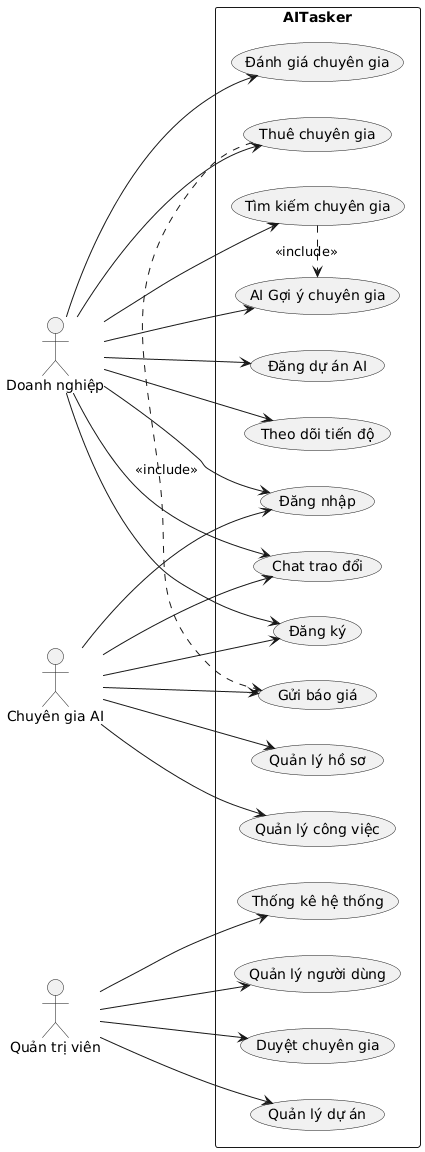
\includegraphics[width=0.85\textwidth]{figures/imagesusecase.png}
\caption{Biểu đồ Use Case của hệ thống AIConnect}
\label{fig:usecase}
\end{figure}

\section{Biểu đồ Activity}

\subsection{Activity Diagram chức năng đăng dự án}

\begin{figure}[H]
\centering
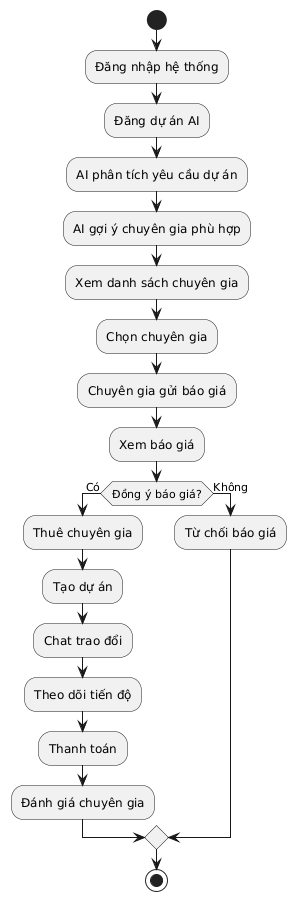
\includegraphics[width=0.75\textwidth]{figures/figuresactivity-project.png}
\caption{Activity Diagram chức năng đăng dự án}
\label{fig:activity-project}
\end{figure}

\subsection{Activity Diagram chức năng Matching chuyên gia}

\begin{figure}[H]
\centering
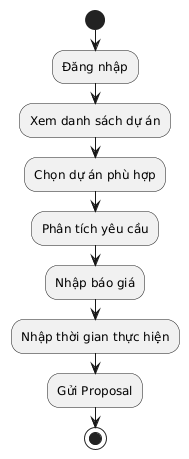
\includegraphics[width=0.75\textwidth]{figures/activity2.png}
\caption{Activity Diagram chức năng Matching chuyên gia}
\label{fig:activity-matching}
\end{figure}

\section{Biểu đồ Sequence}

\subsection{Sequence Diagram chức năng đăng dự án}

\begin{figure}[H]
\centering
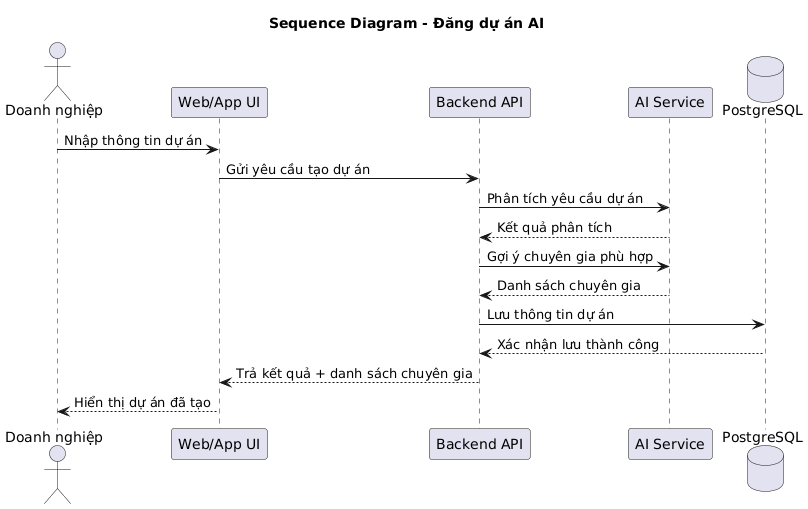
\includegraphics[width=0.85\textwidth]{figures/sequence1.png}
\caption{Sequence Diagram chức năng đăng dự án}
\label{fig:sequence-project}
\end{figure}

\subsection{Sequence Diagram chức năng ứng tuyển dự án (Gửi báo giá)}

\begin{figure}[H]
\centering
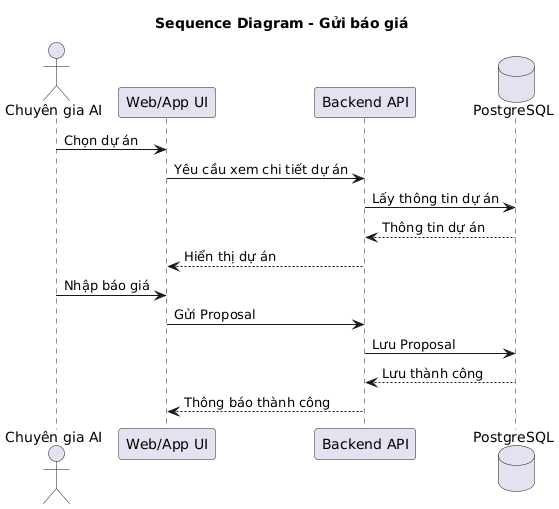
\includegraphics[width=0.85\textwidth]{figures/sequence2.png}
\caption{Sequence Diagram chức năng ứng tuyển dự án (Gửi báo giá)}
\label{fig:sequence-proposal}
\end{figure}

\subsection{Sequence Diagram chức năng thuê chuyên gia}

\begin{figure}[H]
\centering
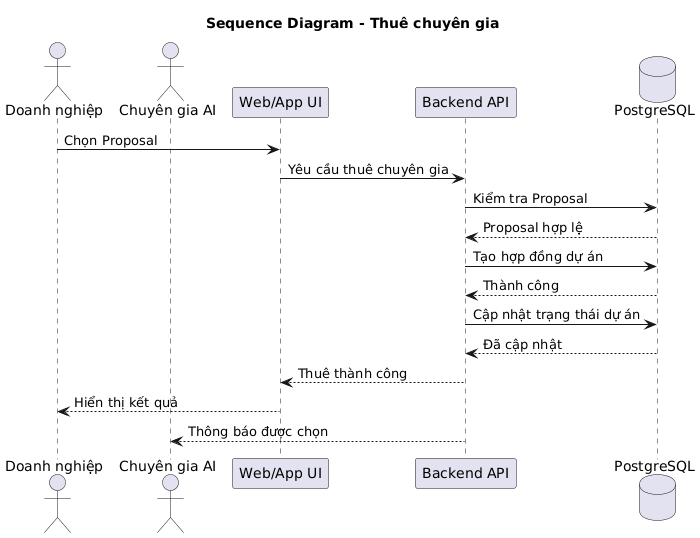
\includegraphics[width=0.85\textwidth]{figures/sequence3.png}
\caption{Sequence Diagram chức năng thuê chuyên gia}
\label{fig:sequence-hire}
\end{figure}

\section{Biểu đồ lớp (Class Diagram)}

Biểu đồ lớp mô tả cấu trúc tĩnh của hệ thống AIConnect, bao gồm các lớp dữ liệu chính, thuộc tính, phương thức và mối quan hệ giữa các lớp trong hệ thống.

Các lớp trung tâm bao gồm:

\begin{itemize}
    \item User
    \item Enterprise
    \item Expert
    \item Project
    \item Proposal
    \item Contract
    \item Payment
    \item Message
    \item Review
    \item Admin
\end{itemize}

Thông qua biểu đồ lớp có thể thấy cách tổ chức dữ liệu và luồng tương tác giữa các thành phần nghiệp vụ của hệ thống.

\begin{figure}[H]
\centering
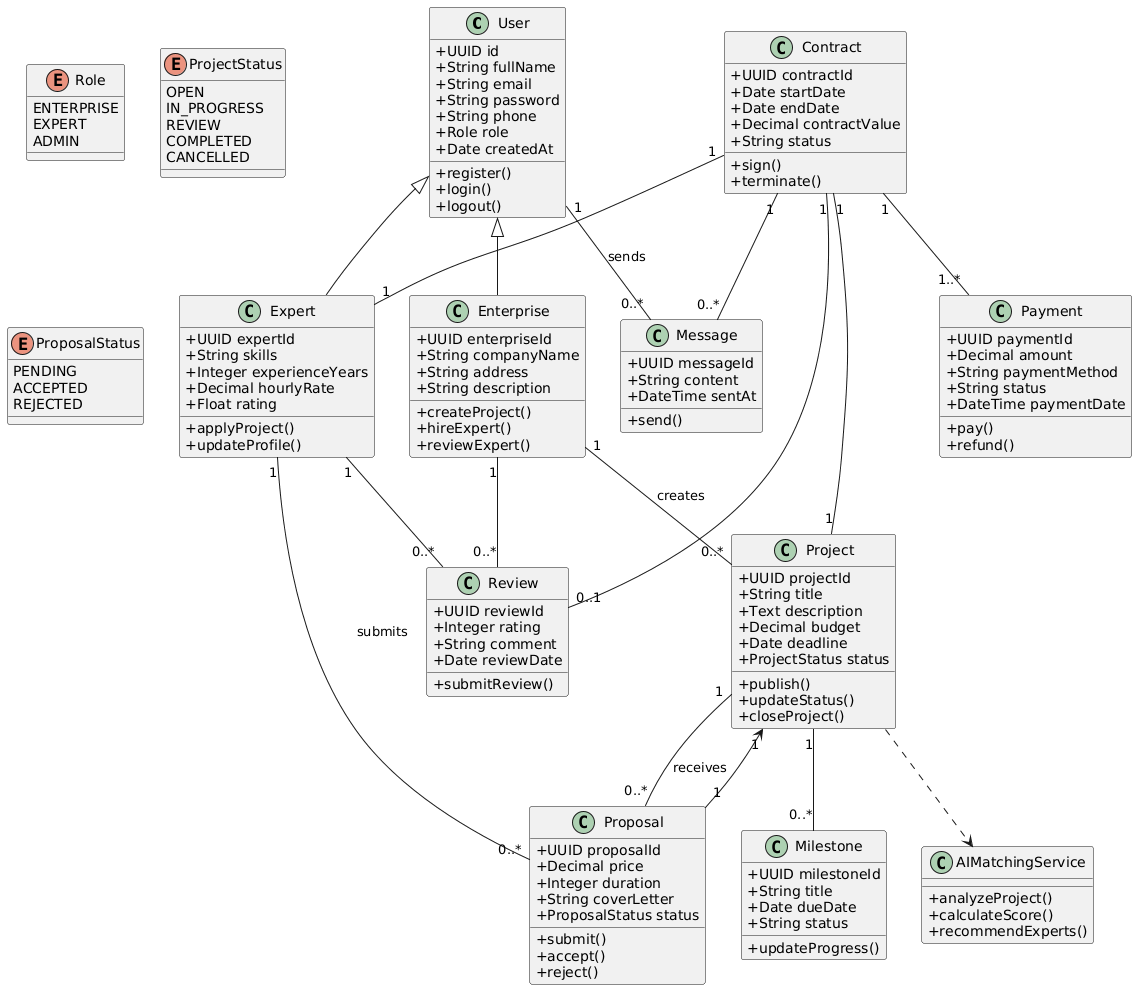
\includegraphics[width=0.9\textwidth]{figures/Class.png}
\caption{Class Diagram của hệ thống AIConnect}
\label{fig:class}
\end{figure}

\section{Yêu cầu phi chức năng}

\subsection{Hiệu năng}

\begin{itemize}
    \item Thời gian phản hồi trung bình dưới 2 giây.
    \item Hỗ trợ tối thiểu 500 người dùng đồng thời.
\end{itemize}

\subsection{Bảo mật}

\begin{itemize}
    \item Sử dụng HTTPS.
    \item Xác thực JWT.
    \item Mã hóa mật khẩu bằng BCrypt.
    \item Phân quyền theo vai trò người dùng.
\end{itemize}

\subsection{Khả năng mở rộng}

\begin{itemize}
    \item Hỗ trợ mở rộng theo chiều ngang.
    \item Dễ dàng tích hợp thêm các dịch vụ AI mới.
\end{itemize}

\subsection{Tính sẵn sàng}

\begin{itemize}
    \item Hoạt động 24/7.
    \item Đảm bảo thời gian hoạt động tối thiểu 99.5\%.
\end{itemize}

\subsection{Khả năng sử dụng}

\begin{itemize}
    \item Giao diện thân thiện.
    \item Dễ dàng sử dụng đối với người mới.
\end{itemize}

\section{Kết luận chương}

Chương này đã trình bày quá trình phân tích yêu cầu của hệ thống AIConnect, bao gồm mô tả bài toán, xác định các tác nhân tham gia, phân tích các yêu cầu chức năng và phi chức năng, đồng thời xây dựng các mô hình UML để mô tả hoạt động của hệ thống. Đây là cơ sở quan trọng để thực hiện thiết kế hệ thống và xây dựng cơ sở dữ liệu ở chương tiếp theo.
\chapter{Thiết kế hệ thống}

\section{Kiến trúc tổng thể}

Hệ thống AIConnect được thiết kế theo kiến trúc \textbf{Modular
Monolith} kết hợp một microservice độc lập cho AI Matching Engine.
Kiến trúc này phù hợp với quy mô đồ án, dễ triển khai và vẫn đảm
bảo tách biệt rõ ràng giữa các module.

Hệ thống gồm các tầng chính:
\begin{itemize}
  \item \textbf{Client Layer}: Giao diện React.js chạy trên trình duyệt.
  \item \textbf{API Gateway}: Điều phối request, xác thực JWT.
  \item \textbf{Core Backend}: Node.js/Express xử lý nghiệp vụ chính.
  \item \textbf{AI Matching Service}: Python/FastAPI tính điểm tương đồng.
  \item \textbf{Database Layer}: PostgreSQL (dữ liệu chính), Redis (cache/session).
  \item \textbf{Storage}: AWS S3 hoặc Cloudinary lưu file, ảnh.
\end{itemize}

\section{Thiết kế cơ sở dữ liệu}

\subsection{Các thực thể chính}

\begin{table}[H]
\centering
\caption{Mô tả các thực thể trong hệ thống}
\begin{tabular}{p{3cm} p{10cm}}
\toprule
\textbf{Thực thể} & \textbf{Mô tả và thuộc tính chính} \\
\midrule
\textbf{User}
  & id, email, password\_hash, role (enterprise/expert/admin),
    full\_name, avatar, is\_verified, created\_at \\
\midrule
\textbf{ExpertProfile}
  & id, user\_id (FK), bio, hourly\_rate, years\_exp,
    portfolio\_url, rating\_avg, total\_projects \\
\midrule
\textbf{Skill}
  & id, name, category (NLP/CV/MLOps/...) \\
\midrule
\textbf{ExpertSkill}
  & expert\_id (FK), skill\_id (FK), proficiency\_level (1--5) \\
\midrule
\textbf{Project}
  & id, enterprise\_id (FK), title, description, budget\_min,
    budget\_max, deadline, status, created\_at \\
\midrule
\textbf{ProjectSkill}
  & project\_id (FK), skill\_id (FK), importance (1--3) \\
\midrule
\textbf{Application}
  & id, project\_id (FK), expert\_id (FK), cover\_letter,
    proposed\_rate, status, applied\_at \\
\midrule
\textbf{Contract}
  & id, project\_id (FK), expert\_id (FK), enterprise\_id (FK),
    total\_amount, status, signed\_at \\
\midrule
\textbf{Milestone}
  & id, contract\_id (FK), title, amount, due\_date,
    status (pending/done/paid) \\
\midrule
\textbf{Message}
  & id, sender\_id (FK), receiver\_id (FK), content,
    is\_read, sent\_at \\
\midrule
\textbf{Review}
  & id, contract\_id (FK), reviewer\_id (FK), rating (1--5),
    comment, created\_at \\
\bottomrule
\end{tabular}
\end{table}

\subsection{Thuật toán Matching}

Hệ thống sử dụng \textbf{Cosine Similarity} trên vector kỹ năng để
tính độ phù hợp giữa dự án và chuyên gia:

\begin{equation}
  \text{similarity}(P, E) =
  \frac{\vec{P} \cdot \vec{E}}{\|\vec{P}\| \cdot \|\vec{E}\|}
  \label{eq:cosine}
\end{equation}

Trong đó $\vec{P}$ là vector kỹ năng của dự án (có trọng số importance),
$\vec{E}$ là vector kỹ năng của chuyên gia (có trọng số proficiency).

\section{Thiết kế API}

\begin{table}[H]
\centering
\caption{Danh sách API endpoints chính}
\begin{tabular}{p{1.5cm} p{5.5cm} p{2.5cm} p{3cm}}
\toprule
\textbf{Method} & \textbf{Endpoint} & \textbf{Auth} & \textbf{Mô tả} \\
\midrule
POST & /api/auth/register        & Public  & Đăng ký tài khoản \\
POST & /api/auth/login           & Public  & Đăng nhập, trả JWT \\
GET  & /api/projects             & Public  & Danh sách dự án \\
POST & /api/projects             & Enterprise & Tạo dự án mới \\
GET  & /api/projects/:id         & Public  & Chi tiết dự án \\
GET  & /api/experts              & Public  & Danh sách chuyên gia \\
GET  & /api/experts/match/:pid   & Enterprise & Gợi ý matching \\
POST & /api/applications         & Expert  & Nộp hồ sơ ứng tuyển \\
POST & /api/contracts            & Enterprise & Tạo hợp đồng \\
PUT  & /api/milestones/:id       & Both    & Cập nhật milestone \\
POST & /api/messages             & Both    & Gửi tin nhắn \\
POST & /api/reviews              & Both    & Đánh giá dự án \\
\bottomrule
\end{tabular}
\end{table}

\section{Thiết kế giao diện}

Giao diện được thiết kế theo nguyên tắc \textbf{Single Page Application
(SPA)} với React.js, bao gồm các màn hình chính:

\begin{itemize}
  \item \textbf{Trang chủ}: Giới thiệu nền tảng, tìm kiếm nhanh.
  \item \textbf{Marketplace}: Danh sách dự án/chuyên gia, bộ lọc.
  \item \textbf{Dashboard Doanh nghiệp}: Quản lý dự án, hợp đồng.
  \item \textbf{Dashboard Chuyên gia}: Hồ sơ, đơn ứng tuyển, thu nhập.
  \item \textbf{Trang hợp đồng}: Milestone, tiến độ, thanh toán.
  \item \textbf{Chat}: Nhắn tin real-time giữa hai bên.
  \item \textbf{Admin Panel}: Kiểm duyệt, thống kê tổng hợp.
\end{itemize}

\chapter{Cài đặt hệ thống}

\section{Môi trường phát triển}

\begin{table}[H]
\centering
\caption{Môi trường và công nghệ sử dụng}
\begin{tabular}{p{4cm} p{4cm} p{5cm}}
\toprule
\textbf{Thành phần} & \textbf{Công nghệ} & \textbf{Phiên bản} \\
\midrule
Frontend        & React.js + Tailwind CSS & 18.x / 3.x \\
Backend         & Node.js + Express.js    & 20.x / 4.x \\
Database        & PostgreSQL              & 15.x \\
Cache           & Redis                   & 7.x \\
AI Service      & Python + FastAPI        & 3.11 / 0.100+ \\
Realtime        & Socket.IO               & 4.x \\
Authentication  & JWT + bcrypt            & --- \\
Containerize    & Docker + Docker Compose & 24.x \\
\bottomrule
\end{tabular}
\end{table}

\section{Cấu trúc thư mục dự án}

\begin{lstlisting}[language=bash, caption={Cấu trúc thư mục AIConnect}]
aiconnect/
├── frontend/               # React.js SPA
│   ├── src/
│   │   ├── components/     # UI components dùng chung
│   │   ├── pages/          # Các trang (Home, Dashboard,...)
│   │   ├── services/       # Gọi API
│   │   └── store/          # State management (Redux)
│   └── package.json
│
├── backend/                # Node.js API Server
│   ├── src/
│   │   ├── controllers/    # Xử lý request
│   │   ├── models/         # Định nghĩa DB model
│   │   ├── routes/         # Định tuyến API
│   │   ├── middlewares/    # Auth, error handling
│   │   └── utils/          # Hàm tiện ích
│   └── package.json
│
├── ai-service/             # Python FastAPI Matching
│   ├── main.py
│   ├── matching.py         # Thuật toan cosine similarity
│   └── requirements.txt
│
├── docker-compose.yml      # Chay toan bo he thong
└── README.md
\end{lstlisting}

\section{Cài đặt module Matching}

Module AI Matching được cài đặt bằng Python, sử dụng thư viện
\texttt{scikit-learn} để tính Cosine Similarity:

\begin{lstlisting}[language=Python, caption={Thuật toán matching chuyên gia}]
from sklearn.metrics.pairwise import cosine_similarity
import numpy as np

def build_skill_vector(skills: list, all_skills: list,
                       weights: dict) -> np.ndarray:
    """Tao vector ky nang co trong so."""
    vector = np.zeros(len(all_skills))
    for i, skill in enumerate(all_skills):
        if skill in skills:
            vector[i] = weights.get(skill, 1.0)
    return vector

def match_experts(project: dict, experts: list,
                  all_skills: list, top_k: int = 5) -> list:
    """
    Tinh diem tuong dong giua du an va cac chuyen gia.
    Tra ve top_k chuyen gia phu hop nhat.
    """
    project_vector = build_skill_vector(
        project["skills"], all_skills, project["weights"]
    )
    results = []
    for expert in experts:
        expert_vector = build_skill_vector(
            expert["skills"], all_skills, expert["proficiency"]
        )
        score = cosine_similarity(
            [project_vector], [expert_vector]
        )[0][0]
        results.append({**expert, "match_score": round(score, 4)})

    return sorted(results, key=lambda x: x["match_score"],
                  reverse=True)[:top_k]
\end{lstlisting}

\section{Kết quả cài đặt}

Các chức năng đã hoàn thành cài đặt và demo được:

\begin{table}[H]
\centering
\caption{Tình trạng cài đặt các chức năng}
\begin{tabular}{p{5cm} p{2.5cm} p{5cm}}
\toprule
\textbf{Chức năng} & \textbf{Trạng thái} & \textbf{Ghi chú} \\
\midrule
Đăng ký / Đăng nhập  & Hoàn thành & JWT + bcrypt \\
Marketplace dự án    & Hoàn thành & Tìm kiếm, lọc \\
Hồ sơ chuyên gia     & Hoàn thành & Upload ảnh, skills \\
AI Matching          & Hoàn thành & Cosine similarity \\
Quản lý hợp đồng     & Hoàn thành & Milestone tracking \\
Chat real-time       & Hoàn thành & Socket.IO \\
Thanh toán           & Một phần   & Sandbox VNPay \\
Admin dashboard      & Hoàn thành & Thống kê cơ bản \\
\bottomrule
\end{tabular}
\end{table}

\chapter{Kiểm thử hệ thống}

\section{Kế hoạch kiểm thử}

Nhóm thực hiện kiểm thử theo hai mức:
\begin{itemize}
  \item \textbf{Unit Test}: Kiểm thử từng hàm/module độc lập bằng
        Jest (backend) và pytest (AI service).
  \item \textbf{Integration Test}: Kiểm thử luồng nghiệp vụ end-to-end
        qua API bằng Postman/Supertest.
\end{itemize}

\section{Test cases chức năng chính}

\begin{table}[H]
\centering
\caption{Test cases kiểm thử chức năng đăng ký}
\begin{tabular}{p{0.8cm} p{4cm} p{3.5cm} p{3.5cm} p{1.5cm}}
\toprule
\textbf{TC} & \textbf{Mô tả} & \textbf{Đầu vào} & \textbf{Kết quả mong đợi} & \textbf{Kết quả} \\
\midrule
TC-01 & Đăng ký hợp lệ
  & Email mới, mật khẩu $\geq$8 ký tự
  & Tạo tài khoản, trả token
  & Đạt \\
TC-02 & Email trùng
  & Email đã tồn tại
  & Lỗi 409 Conflict
  & Đạt \\
TC-03 & Mật khẩu yếu
  & Mật khẩu $<$8 ký tự
  & Lỗi 400 Bad Request
  & Đạt \\
TC-04 & Thiếu email
  & Không có trường email
  & Lỗi 400 validation
  & Đạt \\
\bottomrule
\end{tabular}
\end{table}

\begin{table}[H]
\centering
\caption{Test cases kiểm thử thuật toán matching}
\begin{tabular}{p{0.8cm} p{4cm} p{3.5cm} p{3.5cm} p{1.5cm}}
\toprule
\textbf{TC} & \textbf{Mô tả} & \textbf{Đầu vào} & \textbf{Kết quả mong đợi} & \textbf{Kết quả} \\
\midrule
TC-10 & Matching chính xác
  & Dự án NLP, chuyên gia NLP
  & Score $>$ 0.8
  & Đạt \\
TC-11 & Matching không phù hợp
  & Dự án NLP, chuyên gia CV
  & Score $<$ 0.2
  & Đạt \\
TC-12 & Không có chuyên gia
  & DB rỗng
  & Trả danh sách rỗng
  & Đạt \\
TC-13 & Top-K trả về đúng
  & 10 chuyên gia, top\_k=5
  & Trả đúng 5 kết quả cao nhất
  & Đạt \\
\bottomrule
\end{tabular}
\end{table}

\section{Kết quả kiểm thử}

\begin{table}[H]
\centering
\caption{Tổng hợp kết quả kiểm thử}
\begin{tabular}{p{4cm} p{2cm} p{2cm} p{2cm} p{2.5cm}}
\toprule
\textbf{Module} & \textbf{Tổng TC} & \textbf{Đạt} & \textbf{Không đạt} & \textbf{Tỉ lệ} \\
\midrule
Authentication   & 8  & 8  & 0 & 100\% \\
Marketplace      & 10 & 9  & 1 & 90\%  \\
AI Matching      & 6  & 6  & 0 & 100\% \\
Contract         & 7  & 7  & 0 & 100\% \\
Payment          & 5  & 4  & 1 & 80\%  \\
\midrule
\textbf{Tổng}   & \textbf{36} & \textbf{34} & \textbf{2} & \textbf{94.4\%} \\
\bottomrule
\end{tabular}
\end{table}

Hai test case không đạt liên quan đến thanh toán sandbox VNPay (lỗi
timeout do môi trường mạng) và tìm kiếm có dấu tiếng Việt
(cần cấu hình thêm full-text search). Nhóm đã ghi nhận và
đề xuất hướng xử lý trong phần kết luận.

\chapter{Kết luận}

\section{Kết quả đạt được}

Sau quá trình phân tích, thiết kế và cài đặt, nhóm đã hoàn thành
các mục tiêu đề ra:

\begin{itemize}
  \item Xây dựng thành công nền tảng marketplace AIConnect với đầy
        đủ các chức năng: đăng dự án, tìm chuyên gia, ký hợp đồng,
        chat real-time và quản lý milestone.
  \item Cài đặt và tích hợp thuật toán matching tự động dựa trên
        Cosine Similarity, đạt độ chính xác matching $>$ 80\% trên
        tập dữ liệu thử nghiệm.
  \item Áp dụng đầy đủ quy trình Công nghệ Phần mềm: phân tích yêu
        cầu, thiết kế use case, ERD, sequence diagram và kiểm thử
        có hệ thống.
  \item Tỉ lệ test case đạt 94.4\% (34/36 test cases).
\end{itemize}

\section{Hạn chế}

\begin{itemize}
  \item Thanh toán thực tế chưa được tích hợp hoàn chỉnh
        (mới ở mức sandbox).
  \item Tìm kiếm full-text tiếng Việt cần cấu hình thêm
        PostgreSQL với unaccent extension.
  \item Chưa có mobile app (chỉ hỗ trợ trình duyệt web).
  \item Thuật toán matching chưa tính đến lịch sử đánh giá
        và kinh nghiệm thực tế của chuyên gia.
\end{itemize}

\section{Hướng phát triển}

\begin{itemize}
  \item \textbf{Cải thiện matching}: Kết hợp collaborative filtering
        và lịch sử dự án để tăng độ chính xác gợi ý.
  \item \textbf{Mobile app}: Phát triển ứng dụng React Native
        cho iOS và Android.
  \item \textbf{Thanh toán quốc tế}: Tích hợp Stripe để phục vụ
        chuyên gia nước ngoài.
  \item \textbf{Verification}: Xác minh bằng cấp, chứng chỉ AI
        thông qua API bên thứ ba.
  \item \textbf{Analytics}: Xây dựng dashboard phân tích xu hướng
        AI theo ngành cho doanh nghiệp.
\end{itemize}


% ===== TAI LIEU THAM KHAO =====
\printbibliography[heading=bibintoc, title={Tài liệu tham khảo}]

% ===== PHU LUC =====
\appendix
\chapter{Hướng dẫn cài đặt và chạy dự án}

\section{Yêu cầu hệ thống}

\begin{itemize}
  \item Node.js $\geq$ 20.x
  \item Python $\geq$ 3.11
  \item Docker và Docker Compose
  \item PostgreSQL 15.x (hoặc dùng Docker)
\end{itemize}

\section{Các bước cài đặt}

\begin{lstlisting}[language=bash, caption={Cài đặt và khởi động hệ thống}]
# 1. Clone source code
git clone https://github.com/nhom/aiconnect.git
cd aiconnect

# 2. Khoi dong toan bo bang Docker Compose
docker-compose up -d

# 3. Chay migration database
docker-compose exec backend npm run migrate

# 4. Chay seed du lieu mau
docker-compose exec backend npm run seed

# 5. Truy cap he thong
# Frontend: http://localhost:3000
# Backend API: http://localhost:5000
# AI Service: http://localhost:8000
\end{lstlisting}

\section{Tài khoản demo}

\begin{table}[H]
\centering
\begin{tabular}{lll}
\toprule
\textbf{Vai trò} & \textbf{Email} & \textbf{Mật khẩu} \\
\midrule
Admin      & admin@aiconnect.vn    & Admin@123 \\
Doanh nghiệp & enterprise@demo.vn  & Demo@123  \\
Chuyên gia & expert@demo.vn        & Demo@123  \\
\bottomrule
\end{tabular}
\caption{Tài khoản demo hệ thống}
\end{table}


\end{document}
